\documentclass[paper=a4, fontsize=11pt]{scrartcl} % A4 paper and 11pt font size

\usepackage[T1]{fontenc} % Use 8-bit encoding that has 256 glyphs
\usepackage[english]{babel} % English language/hyphenation
\usepackage{amsmath,amsfonts,amsthm} % Math packages
\usepackage{graphicx}

\usepackage{lipsum} % Used for inserting dummy 'Lorem ipsum' text into the template

\usepackage{sectsty} % Allows customizing section commands
\allsectionsfont{\centering \normalfont\scshape} % Make all sections centered, the default font and small caps

\usepackage{fancyhdr} % Custom headers and footers
\pagestyle{fancyplain} % Makes all pages in the document conform to the custom headers and footers
\fancyhead{} % No page header - if you want one, create it in the same way as the footers below
\fancyfoot[L]{} % Empty left footer
\fancyfoot[C]{} % Empty center footer
\fancyfoot[R]{\thepage} % Page numbering for right footer
\renewcommand{\headrulewidth}{0pt} % Remove header underlines
\renewcommand{\footrulewidth}{0pt} % Remove footer underlines
\setlength{\headheight}{13.6pt} % Customize the height of the header

\numberwithin{equation}{section} % Number equations within sections (i.e. 1.1, 1.2, 2.1, 2.2 instead of 1, 2, 3, 4)
\numberwithin{figure}{section} % Number figures within sections (i.e. 1.1, 1.2, 2.1, 2.2 instead of 1, 2, 3, 4)
\numberwithin{table}{section} % Number tables within sections (i.e. 1.1, 1.2, 2.1, 2.2 instead of 1, 2, 3, 4)

\setlength\parindent{0pt} % Removes all indentation from paragraphs - comment this line for an assignment with lots of text

%----------------------------------------------------------------------------------------
%	TITLE SECTION
%----------------------------------------------------------------------------------------

\newcommand{\horrule}[1]{\rule{\linewidth}{#1}} % Create horizontal rule command with 1 argument of height

\title{	
	\normalfont \normalsize 
	\textsc{EC500 - Introduction to Learning From Data} \\ [25pt] % Your university, school and/or department name(s)
	\horrule{0.5pt} \\[0.4cm] % Thin top horizontal rule
	\huge Matlab - 1 \\ % The assignment title
	\horrule{2pt} \\[0.5cm] % Thick bottom horizontal rule
}

\author{Mikhail Andreev} % Your name

\date{\normalsize\today} % Today's date or a custom date

\begin{document}
	
	\maketitle % Print the title
	
	%----------------------------------------------------------------------------------------
	%	PROBLEM 1
	%----------------------------------------------------------------------------------------
	
	\section{Gaussian Discriminant Analysis}
	
	\subsection{Part a}
	Helper functions located in online submission.
	
	\subsection{Part b}
	
	Mean vectors:
	
	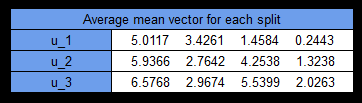
\includegraphics{1b_mean_vectors}
	
	Variances for QDA:
	
	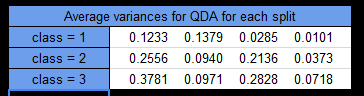
\includegraphics{QDA_variances}
	
	Variances for LDA:
	
	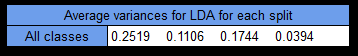
\includegraphics{LDA_variances}
	
	CCR Results:
	
	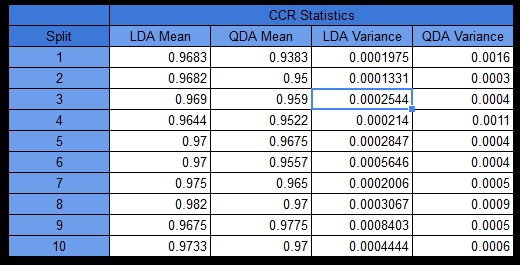
\includegraphics{CCR_Stats}
	
	Confusion matrix of best split in LDA:
	
	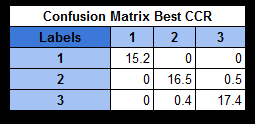
\includegraphics{best_conf_mat}
	
	Confusion matrix of worst split in LDA:
	
	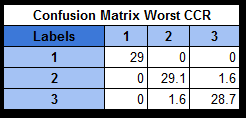
\includegraphics{worst_conf_mat}
	
	\subsection{Part c}
	Helper functions located in online submission.
	
	\subsection{Part d}
	Resulting graph:
	
	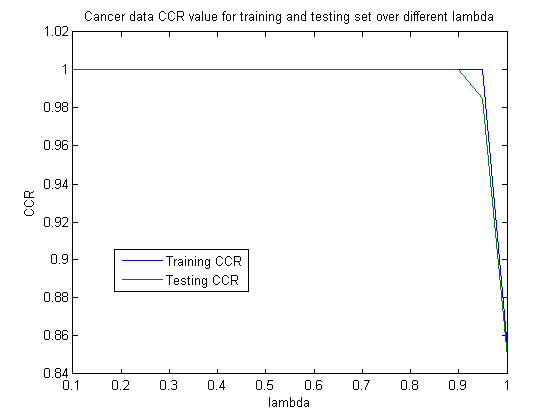
\includegraphics{1d_graph}
	
	%----------------------------------------------------------------------------------------
	%	PROBLEM 2
	%----------------------------------------------------------------------------------------
	
	\section{Naive Bayes Text Document Classifiers}
	
	\subsection{Part a}
	Total number of unique words in training set: 53975

	\par	
	Total number of unique words in testing set: 47376
	
	\par
	Total number of unique words in entire dataset: 61188
	
	\par
	Average document length of training set: 245.39 words.
	
	\par
	Average document length of testing set: 239.43 words.
	
	\par
	Total number of unique words in testing set that are not in the training set: 7213.
	
	\subsection{Part b}
	200778 (16.41\%) $ \beta_{w,c} $'s are non-zero.
	
	\par
	6958 (92.71\%) documents have $ P(Y=c|x) = 0 $ for all $ c = 1,...,20 $. This occurs because the documents contain words that are not seen in the training samples. Since the total probability is the multiplication of all the underlying probabilities for each word, any word in a test sample that has not been seen in a training example for a class, will result in a probability of 0 for that class.
	
	\par
	The test CCR = 5.44\%.
	
	\subsection{Part c}
	200778 (18.60\%) $ \beta_{w,c} $'s are non-zero.
	
	The test CCR = 7.16\%.
	
	\subsection{Part d}
	The test CCR = 78.52\%.
	
	The confusion matrix:
	
	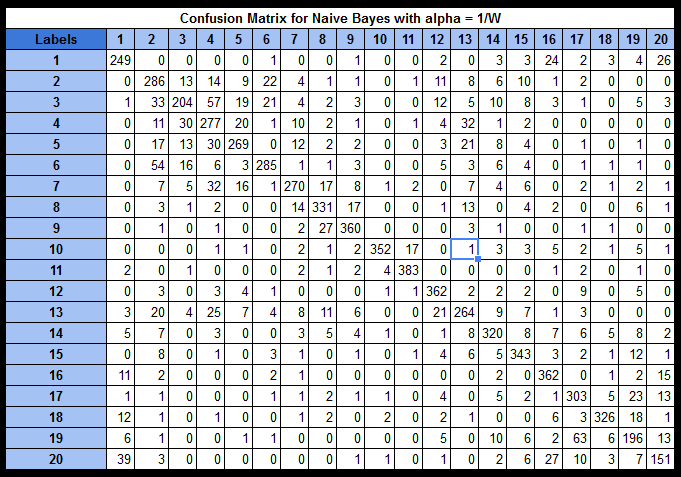
\includegraphics[scale=0.9]{2d_confusion_matrix}
	
	\subsection{Part e}
	
	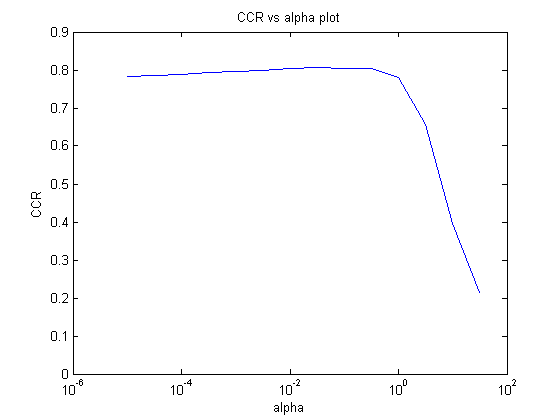
\includegraphics{2e_log_graph}
	
	\subsection{Part f}
	Size of new dictionary: 60698 words.
	
	Average document length of training documents: 116.98 words.
	
	Average document length of testing documents: 114.62 words.
	
	The test CCR = 78.23\%.
		
	%----------------------------------------------------------------------------------------
	%	PROBLEM 3
	%----------------------------------------------------------------------------------------
	
	\section{Nearest Neighbor Classifier}
	
	\subsection{Part a}
	Scatter Plot:
	
	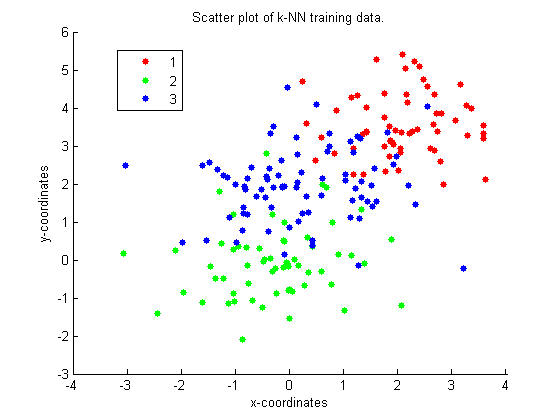
\includegraphics{3_a_scatter_plot}
	
	\subsection{Part b}
	Probability color map for class = 2:
	
	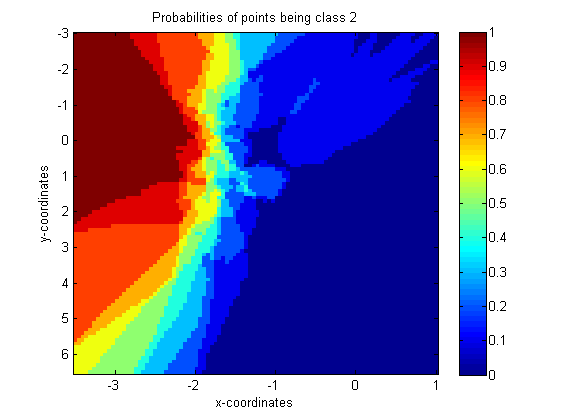
\includegraphics{3b_class2}
	
	Probability color map for class = 3:
	
	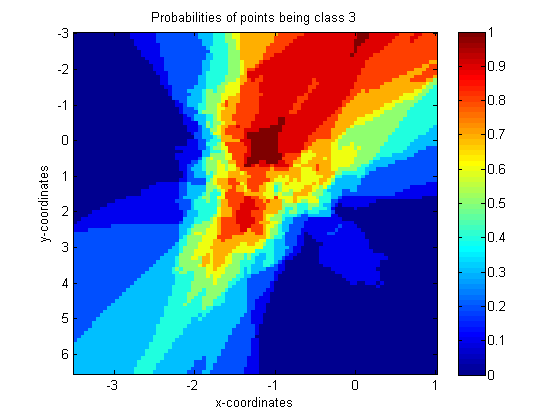
\includegraphics{3b_class3}
	
	\subsection{Part c}
	Classification coding scheme for k = 1:
	
	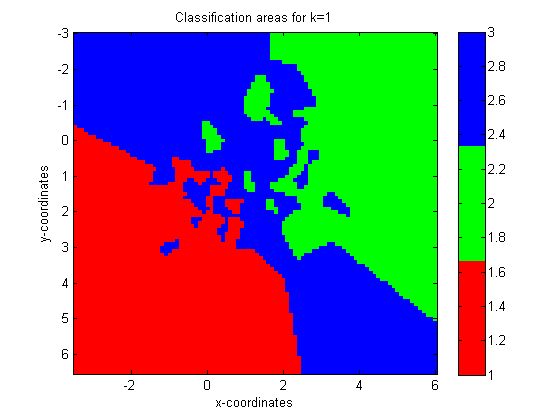
\includegraphics{3c_k1}
	
	Classification coding scheme for k = 5:
	
	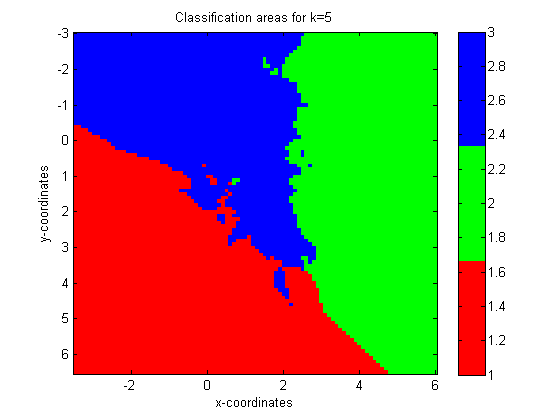
\includegraphics{3c_k5}
	
	Here we can see that for k = 1, we only care about the closest point to each location. Because of this there is a fairly even split between the 3 classes. However, as we expand our search to more points, we see the green and red classes start to dominate as they have more points at close to proximity to much of the area.
	
	\subsection{Part d}
	The Test CCR = 96.31\%
	
	Confusion matrix:
	
	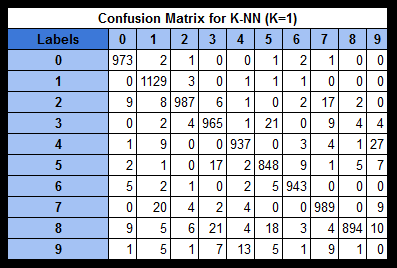
\includegraphics{3d_confusion_matrix}
	
	
\end{document}